\chapter{\ifproject%
\ifcpe การทดลองและผลลัพธ์\else Experimentation and Results\fi
\else%
\ifcpe การประเมินระบบ\else System Evaluation\fi
\fi} \label{eval}

% ในบทนี้จะทดสอบเกี่ยวกับการทำงานในฟังก์ชันหลักๆ
% การทดสอบระบบของเราจะทดสอบโดยใช้ User Test ซึ่งเราจะนำไปให้กลุ่มทดลองที่เป็นเด็กนักเรียนชั้นประถมศึกษาปีที่ 4-6 โรงเรียนรอบนอก
% ชั้นปีละ 20 คนในการทดสอบโดย เราจะวัดผลโดยการใช้ pre-test เพื่อวัดระดับของเด็กนักเรียนก่อนเล่นเกมและ post-test เพื่อวัดระดับของเด็กนักเรียนหลังเล่นเกม
% ซึ่งในเนื้อหา pre-test และ post-test จะเป็นแบบฝึกหัดเนื้อหาวิชาวิทยาการคำนวณ โดยเราจะนำผล pre-test และ post-test มาเทียบกันเพื่อ
% ประเมินตัวเกมของเราว่าจะสามารถเป็นสื่อการเรียนการสอนให้เด็กนักเรียนได้เข้าใจในวิชาวิทยาการคำนวณมากขึ้นจริงไหม 
% รวมไปถึงภายในตัวเกมเองก็จะมีการเก็บ Score ของผู้เล่นโดยแต่ละด่านจะมีจำนวนจำกัดในการใช้ Block Code ซึ่งถ้านักเรียนใช้จำนวนคำสั่งเกินมาจากที่กำหนดไว้คะแนนของนักเรียนจะ
% ลดลงตามจำนวนคำสั่งที่เพิ่มมาและจะมีการเก็บเวลาที่ใช้ในแต่ละด่านของนักเรียนแต่ละคนเดียว ทั้งหมดนี้จะนำไปขึ้น Score Board เพิ่งแสดงให้เห็นว่าตัวนักเรียนเองได้คะแนนจากด่านนี้ๆ เท่าไหร่
% \CIreply{ใจความของย่อหน้านี้คืออะไร
การประเมินระบบของโครงการนี้ จะมีการประเมินอยู่ 2 วิธี ได้แก่วิธี user test โดยเด็กนักเรียนชั้นประถมศึกษาปีที่ 3--6 ผ่านเครื่องมือการ pre-test/post-test และวิธี expert test เพื่อประเมินระบบภายในเกม ความยากง่ายของเกม (game design) และ UX/UI ผ่าน
เครื่องมือที่เรียกว่า IOC

\section{User test}
การศึกษาเรื่องการวัดผลวิชาวิทยาการคำนวณสำหรับนักเรียนชั้นประถมศึกษาปีที่ 3--6 
โรงเรียนบ้านออนใต้และโรงเรียนบ้านโฮ้ง อำเภอสันกำแพง
 จังหวัดเชียงใหม่ โดยใช้การวัดผลแบบ pre-test/post-test ก่อนและหลังเล่นเกม ผู้ศึกษานำเสนอผลวิเคราะห์ข้อมูลตามลำดับดังนี้

\subsection{Pre-test/post-test}
การทดสอบก่อนและหลังเล่นเกมเสริมทักษะวิชาวิทยาการคำนวณของนักเรียนชั้นประถมศึกษาปีที่ 3--6 โรงเรียนบ้านออนใต้ และโรงเรียนบ้านโฮ้ง จะแสดงให้เห็นถึงการเสริมสร้างทักษะการคิดเชิงคำนวณ และการคิดอย่างเป็นขั้นเป็นตอน โดยภายในเกมประกอบไปด้วยด่านจำนวน 30 ด่าน
แต่ละด่านประกอบไปด้วยรายละเอียดดังต่อไปนี้ ตามตารางที่~\ref{mappictable} สามารถดูรายละเอียดและคำอธิบายของแต่ละด่านได้ในภาคผนวกที่~
% \begin{center}
%     \begin{table}[H]
%         \begin{center}
%             \begin{tabularx}{\textwidth}{|c | X|} 
%              \hline
%              ด่านที่ & เนื้อหา\\ [0.5ex] 
%              \hline\hline
%              1 &  ศึกษาวิธีการเล่นเกมโดยให้ตัวละครเดินไป 1 ก้าว \\ 
%              \hline
%              2 &  ศึกษาวิธีการเปลี่ยนค่าในกล่องคำสั่งโดยให้ตัวละครเดินไป 2 ก้าว \\ 
%              \hline
%              3 &  ศึกษาวิธีการเปลี่ยนค่าในกล่องคำสั่งโดยให้ตัวละครเดินไป 4 ก้าว \\ 
%              \hline
%              4 &  ศึกษาคำสั่งใหม่ (หมุน) โดยให้ตัวละครหมุน 1 ครั้งและเดิน 1 ก้าว \\ 
%              \hline
%              5 &  ศึกษาคำสั่งใหม่ (หมุน) โดยให้ตัวละครหมุน 1 ครั้งและเดิน 4 ก้าว \\ 
%              \hline
%              6 &  ผสมผสานคำสั่งโดยให้ตัวละครเดินและหมุน \\ 
%              \hline
%              7 &  ผสมผสานคำสั่งโดยให้ตัวละครเดินและหมุนไปในอีกทิศทาง \\ 
%              \hline
%              8 &  เพิ่มระดับความยากจากด่านก่อนหน้าโดยต้องใช้คำสั่ง หมุนและเดิน มากขึ้น \\ 
%              \hline
%              9 &  เพิ่มระดับความยากจากด่านก่อนหน้าโดยต้องใช้คำสั่ง หมุนและเดิน มากขึ้น \\ 
%              \hline
%              10 &  เพิ่มระดับความยากจากด่านก่อนหน้าโดยต้องใช้คำสั่ง หมุนและเดิน มากขึ้น \\ 
%              \hline
%              11 &  ศึกษาคำสั่งใหม่ (ทำซ้ำ) โดยให้ผู้ใช้เดินไป 1 ก้าวและครอบด้วยคำสั่งทำซ้ำ \\ 
%              \hline
%              12 &  ผสมผสานคำสั่ง เดิน, หมุน และทำซ้ำโดยให้ตัวละครเดินเป็นตัว U คว่ำ \\ 
%              \hline
%              13 &  ผสมผสานคำสั่ง เดิน, หมุน และทำซ้ำโดยให้ตัวละครเดินเป็นซิกเซ็ก \\ 
%              \hline
%              14 &  ผสมผสานคำสั่ง เดิน, หมุน และทำซ้ำโดยให้ตัวละครเดินเป็นตัว U คว่ำที่ใหญ่กว่า \\ 
%              \hline
%              15 &  ผสมผสานคำสั่ง เดิน, หมุน และทำซ้ำโดยให้ตัวละครเดินเป็นตัว U คว่ำ โดยมีการหลอก \\ 
%              \hline
%              16 &  ศึกษาคำสั่งใหม่ (ตัวแปร) \\ 
%              \hline
%              17 &  ศึกษาวิธีเปลี่ยนค่าของคำสั่งตัวแปร \\ 
%              \hline
%              18 &  ผสมผสานคำสั่ง เดิน, ตัวแปร และหมุน \\ 
%              \hline
%              19 &  ผสมผสานคำสั่ง เดิน, ตัวแปร, หมุน และทำซ้ำโดยให้ตัวละครเดินเป็นรูปก้นหอย \\ 
%              \hline
%              20 &  ผสมผสานคำสั่ง เดิน, ตัวแปร, หมุน และทำซ้ำโดยให้ตัวละครเดินเป็นรูปก้นหอยที่ใหญ่ขึ้น \\ 
%              \hline
%              21 &  ศึกษาคำสั่งใหม่ (เหยียบบน block สี) โดยให้เดินไปข้างหน้า \\ 
%              \hline
%              22 &  ผสมผสานคำสั่ง เดิน, หมุน และเหยียบบน block สี \\ 
%              \hline
%              23 &  ผสมผสานคำสั่ง เดิน, หมุน และเหยียบบน block สีโดยมีการเปลี่ยนค่าของคำสั่ง \\ 
%              \hline
%              24 &  ผสมผสานคำสั่ง เดิน, หมุน, เหยียบบน block สี และ ทำซ้ำ \\ 
%              \hline
%              25 &  ผสมผสานคำสั่ง เดิน, หมุน, เหยียบบน block สี และ ทำซ้ำ โดยให้เดินเป็นรูปตัว U คว่ำ \\ 
%              \hline
%              26 &  เพิ่มจำนวน block สีที่เหยียบได้ โดยในด่านจะมี 2 สี \\ 
%              \hline
%              27 &  ผสมผสานคำสั่ง เดิน, หมุน, เหยียบบน block สี และ ทำซ้ำ โดยให้เดินเป็นซิกเซ๊ก \\ 
%              \hline
%              28 &  ผสมผสานคำสั่ง เดิน, หมุน, เหยียบบน block สี และ ทำซ้ำ โดยให้เดินเป็นซิกเซ๊กโดยเพิ่มจำนวนคำสั่งที่ใช้ \\ 
%              \hline
%              29 &  ผสมผสานคำสั่ง เดิน, หมุน, เหยียบบน block สี และ ทำซ้ำ โดยให้เดินเป็นรูปตัว U คว่ำพร้อมทั้งมีการหลอกการใช้คำสั่ง \\ 
%              \hline
%              30 &  ผสมผสานคำสั่ง เดิน, หมุน, เหยียบบน block สี และ ทำซ้ำ โดยมี block สีที่เหยียบได้ 3 สี \\ 
%              \hline
%             \end{tabularx}
%         \end{center}
%         \caption[ตารางข้อมูลแต่ละด่าน]{ตารางข้อมูลแต่ละด่าน}
%         \label{maptable}
%     \end{table}
% \end{center}
\begin{table}[H]
    \begin{center}
        \begin{tabular}{|c | c|}
            \hline
            ด่านที่ & หน้าตาด่าน\\
            \hline\hline
            1 &  ดังรูปที่~\ref{s1} \\ 
            \hline
            2 &  ดังรูปที่~\ref{s2} \\ 
            \hline
            3 &  ดังรูปที่~\ref{s3} \\ 
            \hline
            4 &  ดังรูปที่~\ref{s4} \\ 
            \hline
            5 &  ดังรูปที่~\ref{s5} \\ 
            \hline
            6 &  ดังรูปที่~\ref{s6} \\ 
            \hline
            7 &  ดังรูปที่~\ref{s7} \\ 
            \hline
            8 &  ดังรูปที่~\ref{s8} \\ 
            \hline
            9 &  ดังรูปที่~\ref{s9} \\ 
            \hline
            10 &  ดังรูปที่~\ref{s10} \\ 
            \hline
            11 &  ดังรูปที่~\ref{s11} \\ 
            \hline
            12 &  ดังรูปที่~\ref{s12} \\ 
            \hline
            13 &  ดังรูปที่~\ref{s13} \\ 
            \hline
            14 &  ดังรูปที่~\ref{s14} \\ 
            \hline
            15 &  ดังรูปที่~\ref{s15} \\ 
            \hline
            16 &  ดังรูปที่~\ref{s16} \\ 
            \hline
            17 &  ดังรูปที่~\ref{s17} \\ 
            \hline
            18 &  ดังรูปที่~\ref{s18} \\ 
            \hline
            19 &  ดังรูปที่~\ref{s19} \\ 
            \hline
            20 &  ดังรูปที่~\ref{s20} \\ 
            \hline
            21 &  ดังรูปที่~\ref{s21} \\ 
            \hline
            22 &  ดังรูปที่~\ref{s22} \\ 
            \hline
            23 &  ดังรูปที่~\ref{s23} \\ 
            \hline
            24 &  ดังรูปที่~\ref{s24} \\ 
            \hline
            25 &  ดังรูปที่~\ref{s25} \\ 
            \hline
            26 &  ดังรูปที่~\ref{s26} \\ 
            \hline
            27 &  ดังรูปที่~\ref{s27} \\ 
            \hline
            28 &  ดังรูปที่~\ref{s28} \\ 
            \hline
            29 &  ดังรูปที่~\ref{s29} \\ 
            \hline
            30 &  ดังรูปที่~\ref{s30} \\ 
            \hline
        \end{tabular}
    \end{center}
    \caption[ตารางภาพแต่ละด่าน]{ตารางภาพแต่ละด่าน}
    \label{mappictable}
\end{table}
จากผลการประเมินความเหมาะสมของเกมเสริมทักษะวิชาวิทยาการคำนวณ (Escape) สำหรับนักเรียนชั้นประถมศึกษาปีที่ 
3--6 โรงเรียนบ้านออนใต้ และโรงเรียนบ้านโฮ้ง อำเภอสันกำแพง จังหวัดเชียงใหม่ 
โดยมีผู้เชี่ยวชาญจำนวน 2 ท่าน ผ่านการพูดคุยและปรึกษา จึงได้ปรับแก้เนื้อหาที่อิงตามหลักสูตรวิชาวิทยาการคำนวณภายในด่าน 
ให้เหมาะสมกับศักยภาพและวัยของผู้เรียนดังที่เห็นในตารางข้างต้น และเมื่อนำเกมเสริมทักษะวิชาวิทยาการคำนวณ (Escape) 
ไปใช้กับกลุ่มเป้าหมาย พบประเด็นที่น่าสนใจดังนี้

\begin{enumerate}
    \item นักเรียนมีความกระตือรือร้นในการทำกิจกรรมโดยใช้เกมเสริมทักษะวิชาวิทยาการคำนวณ (Escape) และได้รับสนุกสนานควบคู่ไปกับความรู้ 
    \item เสริมสร้างกระบวนการเรียนรู้ทางเทคโนโลยี และฝึกให้เด็กได้ใช้ความคิดอย่างเป็นขั้นเป็นตอน ตามหลักสูตรแกนกลางการศึกษาขั้นพื้นฐาน พุทธศักราช 2560 ในรายวิชาวิทยาศาสตร์ (วิทยาการคำนวณ)
\end{enumerate}

\subsubsection{ผลการเรียนรู้เรื่องวิชาวิทยาการคำนวณสำหรับนักเรียนชั้นประถมศึกษาปีที่ 3--6 โรงเรียน บ้านออนใต้และโรงเรียนบ้านโฮ้ง อำเภอสันกำแพง จังหวัดเชียงใหม่}

คะแนนจากการทำแบบทดสอบวัดผลการเรียนรู้ของวิชาวิทยาการคำนวณ หมวดหมู่การคิดอย่างเป็นขั้นเป็นตอน โดยใช้เครื่องมือคือเกมเสริมทักษะวิชาวิทยาการคำนวณ (Escape)
\begin{center}
\begin{tikzpicture}
    \begin{axis} [
        xtick={ป.3,ป.4,ป.5,ป.6},  % Use this to decide which tickmarks to print
        xticklabel style={text height=2ex}, % This aligns all letters on the same line, if it is missing, 'a' and 'b' are at different heights
        ymin=0,
        ylabel=คะแนน,
        ymin=0,
        symbolic x coords={ป.3,ป.4,ป.5,ป.6},
        legend style={at={(0.5,-0.1)},
        anchor=north,legend columns=-5},
        width=11cm,
        ybar,
        bar width=7pt,
        ]
        
        \addplot[red!20!black,fill=red!80!white,ybar,fill] coordinates {(ป.3,34) (ป.4,38) (ป.5,67) (ป.6,73)};
        \addplot[blue!20!black,fill=blue!80!white,ybar,fill] coordinates {(ป.3,32) (ป.4,40) (ป.5,84) (ป.6,100)};
        
        \legend {Pre-Test, Post-Test};
     
    \end{axis}
\end{tikzpicture}
\end{center}

จากการทดสอบนักเรียนชั้นประถมศึกษาชั้นปีที่ 3--6 ด้วยข้อสอบวิชาวิทยาการคำนวณก่อนและหลังเล่นเกม นักเรียนทุกคนมีพัฒนาการเพิ่มขึ้นเป็นที่น่าพึงพอใจเมื่อทำข้อสอบที่มีความยากมากขึ้น
\pagebreak
\begin{figure}[H]
    \begin{center}
    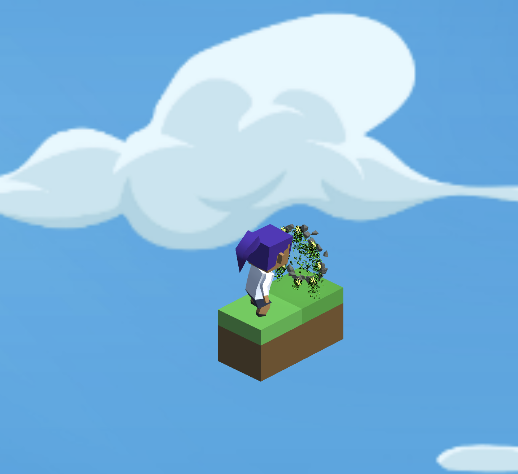
\includegraphics[width=2.5in]{pic-toro/stage/s1.png}
    \end{center}
    \caption[รูปภาพของด่านที่ 1]{รูปภาพของด่านที่ 1}
    \label{s1}
\end{figure}
\begin{figure}[H]
    \begin{center}
    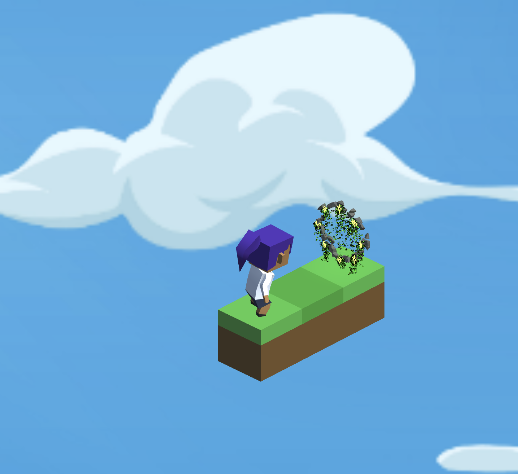
\includegraphics[width=2.5in]{pic-toro/stage/s2.png}
    \end{center}
    \caption[รูปภาพของด่านที่ 2]{รูปภาพของด่านที่ 2}
    \label{s2}
\end{figure}
\begin{figure}[H]
    \begin{center}
    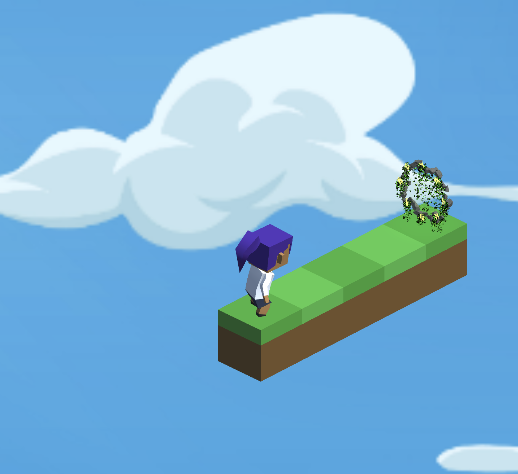
\includegraphics[width=2.5in]{pic-toro/stage/s3.png}
    \end{center}
    \caption[รูปภาพของด่านที่ 3]{รูปภาพของด่านที่ 3}
    \label{s3}
\end{figure}
\begin{figure}[H]
    \begin{center}
    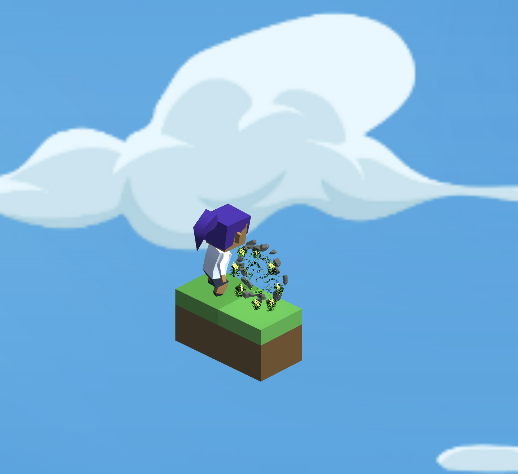
\includegraphics[width=2.5in]{pic-toro/stage/s4.png}
    \end{center}
    \caption[รูปภาพของด่านที่ 4]{รูปภาพของด่านที่ 4}
    \label{s4}
\end{figure}
\begin{figure}[H]
    \begin{center}
    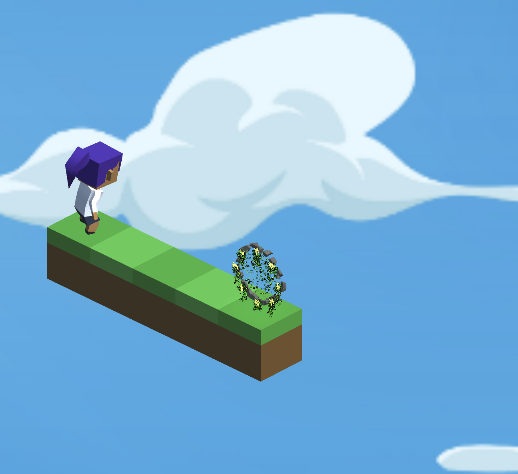
\includegraphics[width=2.5in]{pic-toro/stage/s5.png}
    \end{center}
    \caption[รูปภาพของด่านที่ 5]{รูปภาพของด่านที่ 5}
    \label{s5}
\end{figure}
\begin{figure}[H]
    \begin{center}
    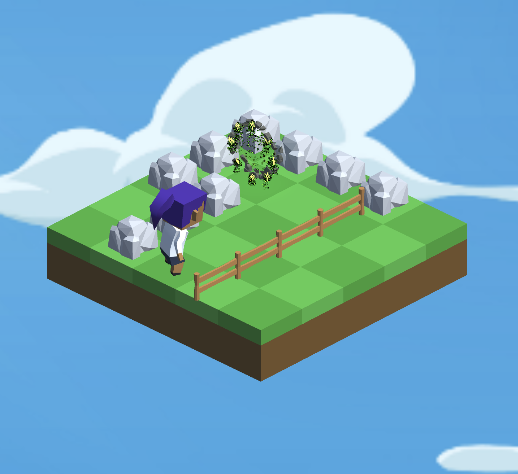
\includegraphics[width=2.5in]{pic-toro/stage/s6.png}
    \end{center}
    \caption[รูปภาพของด่านที่ 6]{รูปภาพของด่านที่ 6}
    \label{s6}
\end{figure}
\begin{figure}[H]
    \begin{center}
    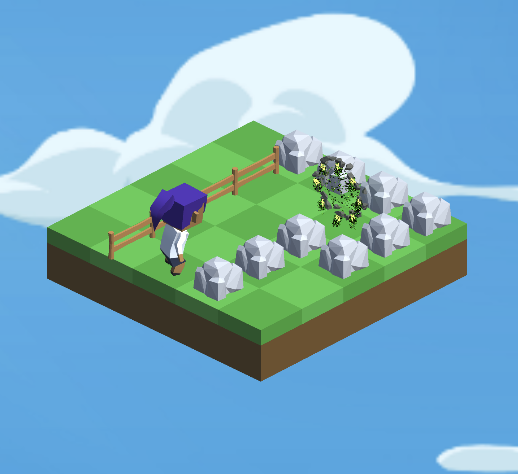
\includegraphics[width=2.5in]{pic-toro/stage/s7.png}
    \end{center}
    \caption[รูปภาพของด่านที่ 7]{รูปภาพของด่านที่ 7}
    \label{s7}
\end{figure}
\begin{figure}[H]
    \begin{center}
    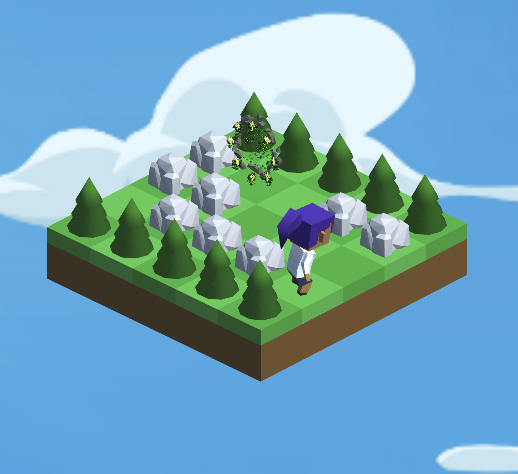
\includegraphics[width=2.5in]{pic-toro/stage/s8.png}
    \end{center}
    \caption[รูปภาพของด่านที่ 8]{รูปภาพของด่านที่ 8}
    \label{s8}
\end{figure}
\begin{figure}[H]
    \begin{center}
    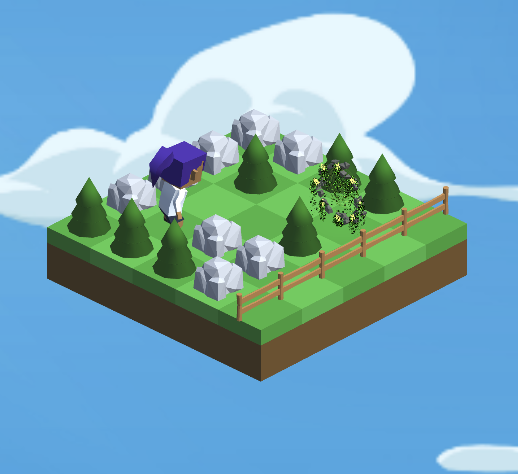
\includegraphics[width=2.5in]{pic-toro/stage/s9.png}
    \end{center}
    \caption[รูปภาพของด่านที่ 9]{รูปภาพของด่านที่ 9}
    \label{s9}
\end{figure}
\begin{figure}[H]
    \begin{center}
    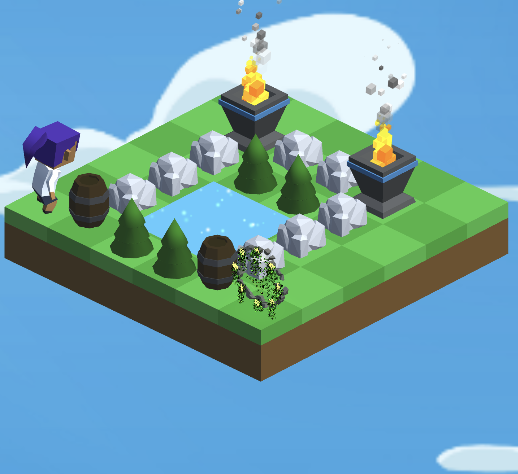
\includegraphics[width=2.5in]{pic-toro/stage/s10.png}
    \end{center}
    \caption[รูปภาพของด่านที่ 10]{รูปภาพของด่านที่ 10}
    \label{s10}
\end{figure}
\begin{figure}[H]
    \begin{center}
    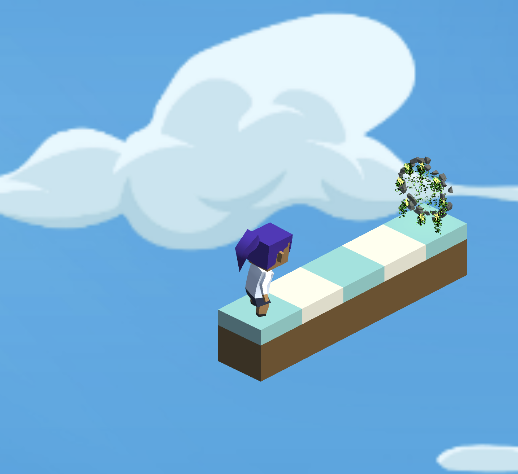
\includegraphics[width=2.5in]{pic-toro/stage/s11.png}
    \end{center}
    \caption[รูปภาพของด่านที่ 11]{รูปภาพของด่านที่ 11}
    \label{s11}
\end{figure}
\begin{figure}[H]
    \begin{center}
    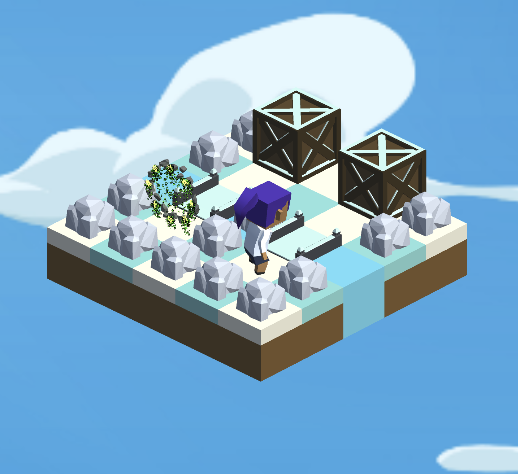
\includegraphics[width=2.5in]{pic-toro/stage/s12.png}
    \end{center}
    \caption[รูปภาพของด่านที่ 12]{รูปภาพของด่านที่ 12}
    \label{s12}
\end{figure}
\begin{figure}[H]
    \begin{center}
    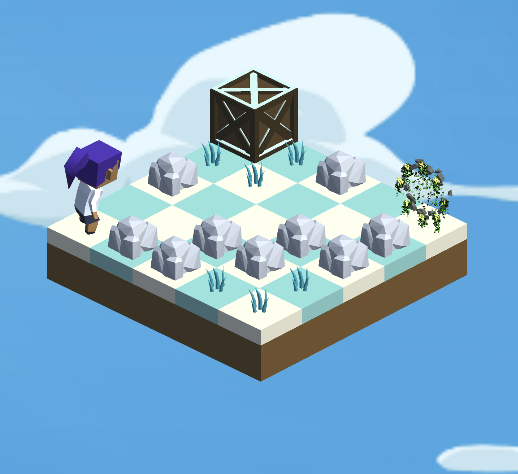
\includegraphics[width=2.5in]{pic-toro/stage/s13.png}
    \end{center}
    \caption[รูปภาพของด่านที่ 13]{รูปภาพของด่านที่ 13}
    \label{s13}
\end{figure}
\begin{figure}[H]
    \begin{center}
    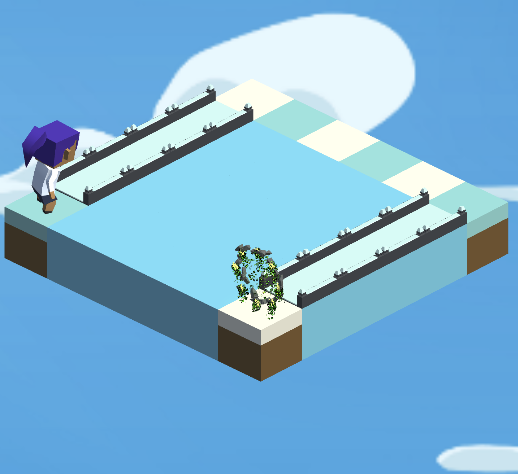
\includegraphics[width=2.5in]{pic-toro/stage/s14.png}
    \end{center}
    \caption[รูปภาพของด่านที่ 14]{รูปภาพของด่านที่ 14}
    \label{s14}
\end{figure}
\begin{figure}[H]
    \begin{center}
    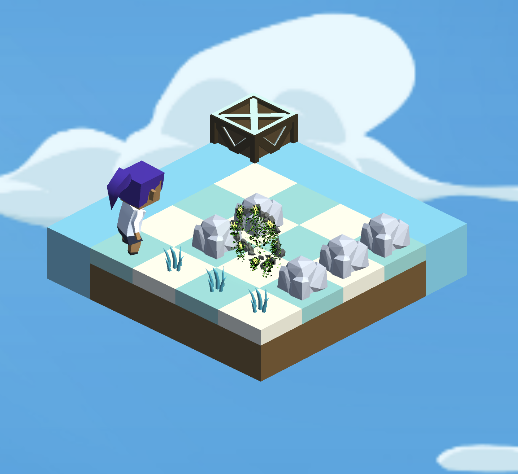
\includegraphics[width=2.5in]{pic-toro/stage/s15.png}
    \end{center}
    \caption[รูปภาพของด่านที่ 15]{รูปภาพของด่านที่ 15}
    \label{s15}
\end{figure}
\begin{figure}[H]
    \begin{center}
    
\includegraphics[width=2.5in]{pic-toro/stage/s16.png}
    \end{center}
    \caption[รูปภาพของด่านที่ 16]{รูปภาพของด่านที่ 16}
    \label{s16}
\end{figure}
\begin{figure}[H]
    \begin{center}
    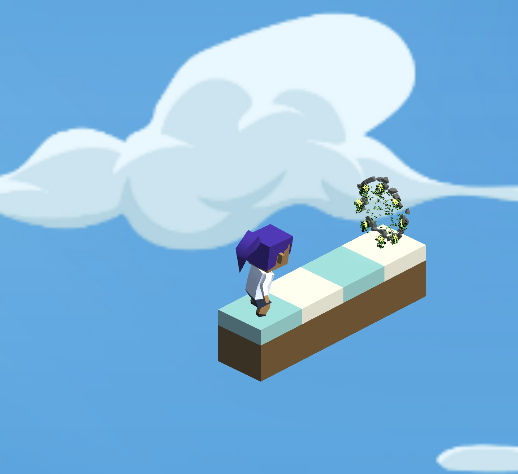
\includegraphics[width=2.5in]{pic-toro/stage/s17.png}
    \end{center}
    \caption[รูปภาพของด่านที่ 17]{รูปภาพของด่านที่ 17}
    \label{s17}
\end{figure}
\begin{figure}[H]
    \begin{center}
    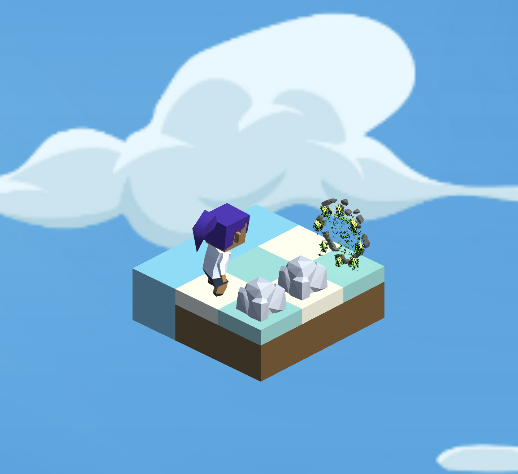
\includegraphics[width=2.5in]{pic-toro/stage/s18.png}
    \end{center}
    \caption[รูปภาพของด่านที่ 18]{รูปภาพของด่านที่ 18}
    \label{s18}
\end{figure}
\begin{figure}[H]
    \begin{center}
    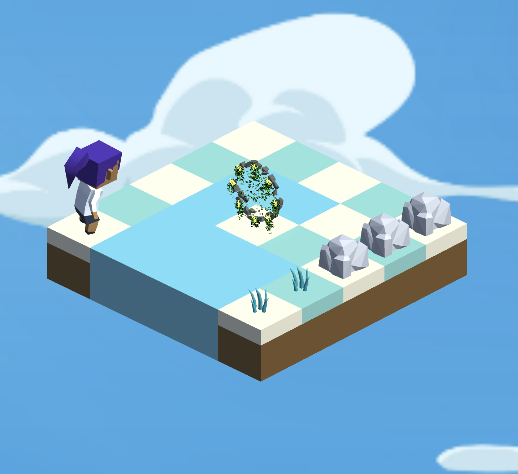
\includegraphics[width=2.5in]{pic-toro/stage/s19.png}
    \end{center}
    \caption[รูปภาพของด่านที่ 19]{รูปภาพของด่านที่ 19}
    \label{s19}
\end{figure}
\begin{figure}[H]
    \begin{center}
    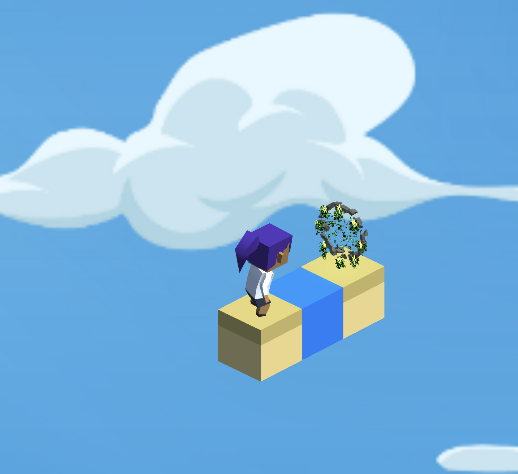
\includegraphics[width=2.5in]{pic-toro/stage/s20.png}
    \end{center}
    \caption[รูปภาพของด่านที่ 20]{รูปภาพของด่านที่ 20}
    \label{s20}
\end{figure}
\begin{figure}[H]
    \begin{center}
    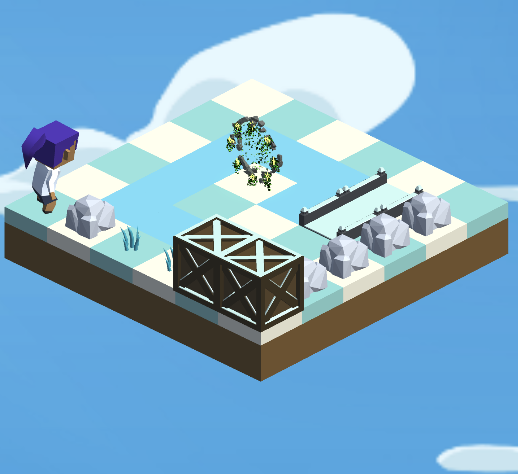
\includegraphics[width=2.5in]{pic-toro/stage/s21.png}
    \end{center}
    \caption[รูปภาพของด่านที่ 21]{รูปภาพของด่านที่ 21}
    \label{s21}
\end{figure}
\begin{figure}[H]
    \begin{center}
    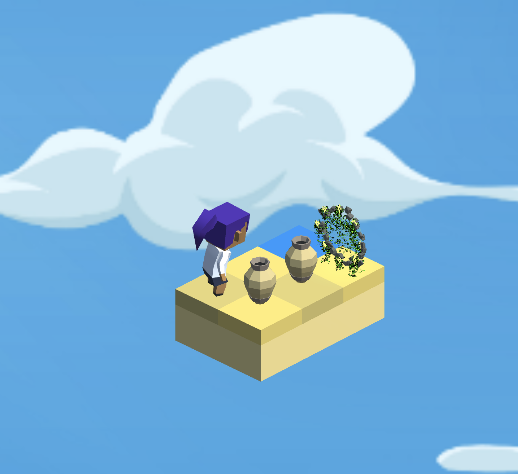
\includegraphics[width=2.5in]{pic-toro/stage/s22.png}
    \end{center}
    \caption[รูปภาพของด่านที่ 22]{รูปภาพของด่านที่ 22}
    \label{s22}
\end{figure}
\begin{figure}[H]
    \begin{center}
    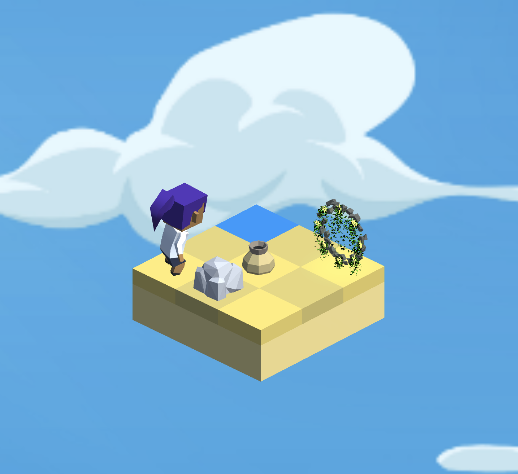
\includegraphics[width=2.5in]{pic-toro/stage/s23.png}
    \end{center}
    \caption[รูปภาพของด่านที่ 23]{รูปภาพของด่านที่ 23}
    \label{s23}
\end{figure}
\begin{figure}[H]
    \begin{center}
    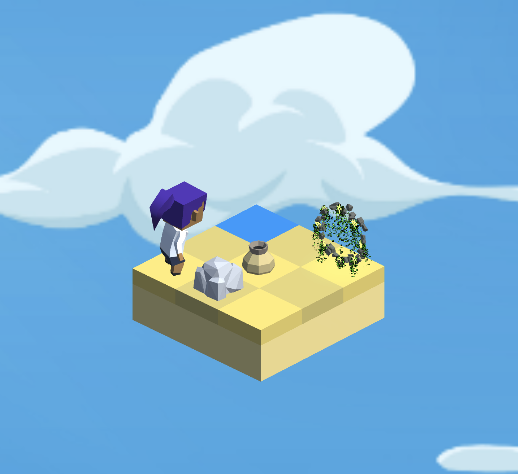
\includegraphics[width=2.5in]{pic-toro/stage/s24.png}
    \end{center}
    \caption[รูปภาพของด่านที่ 24]{รูปภาพของด่านที่ 24}
    \label{s24}
\end{figure}
\begin{figure}[H]
    \begin{center}
    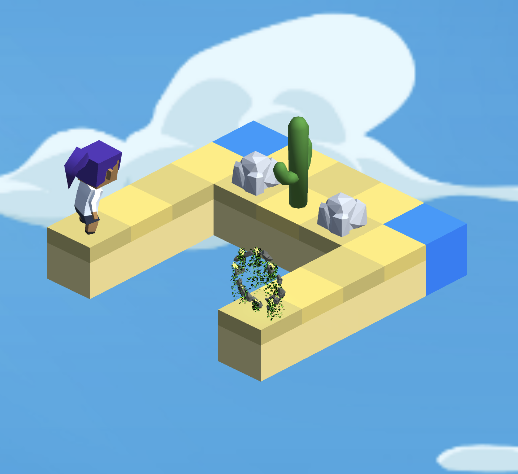
\includegraphics[width=2.5in]{pic-toro/stage/s25.png}
    \end{center}
    \caption[รูปภาพของด่านที่ 25]{รูปภาพของด่านที่ 25}
    \label{s25}
\end{figure}
\begin{figure}[H]
    \begin{center}
    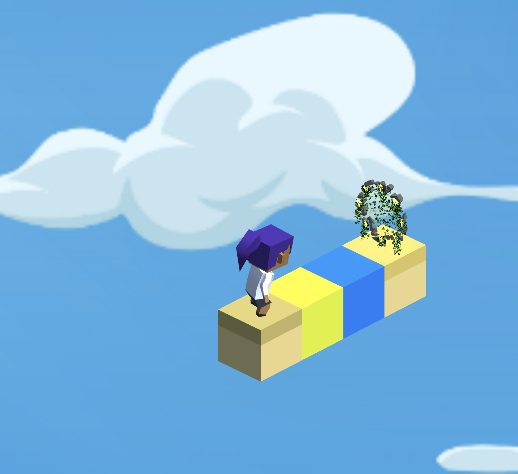
\includegraphics[width=2.5in]{pic-toro/stage/s26.png}
    \end{center}
    \caption[รูปภาพของด่านที่ 26]{รูปภาพของด่านที่ 26}
    \label{s26}
\end{figure}
\begin{figure}[H]
    \begin{center}
    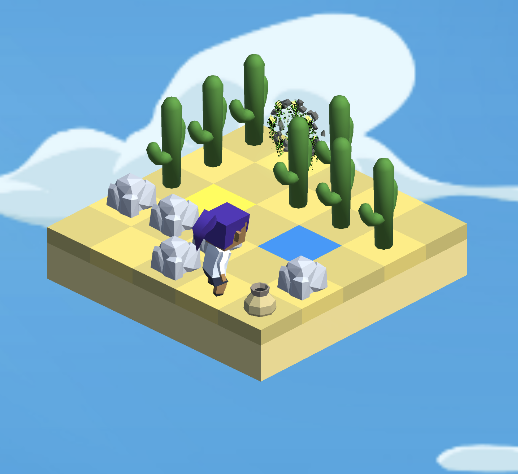
\includegraphics[width=2.5in]{pic-toro/stage/s27.png}
    \end{center}
    \caption[รูปภาพของด่านที่ 27]{รูปภาพของด่านที่ 27}
    \label{s27}
\end{figure}
\begin{figure}[H]
    \begin{center}
    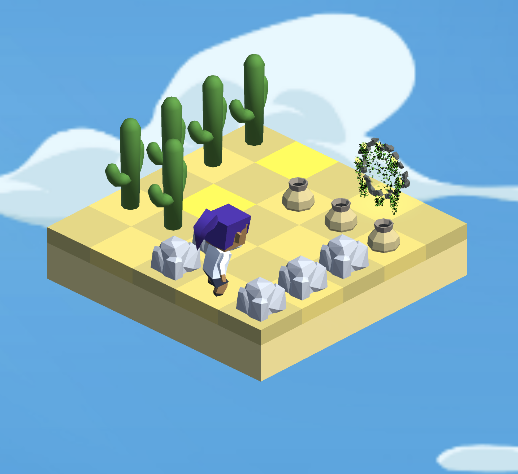
\includegraphics[width=2.5in]{pic-toro/stage/s28.png}
    \end{center}
    \caption[รูปภาพของด่านที่ 28]{รูปภาพของด่านที่ 28}
    \label{s28}
\end{figure}
\begin{figure}[H]
    \begin{center}
    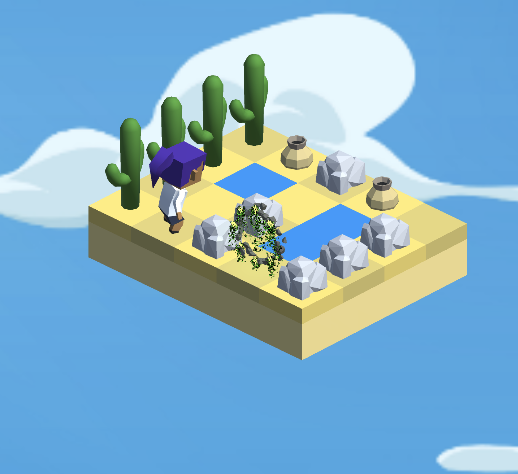
\includegraphics[width=2.5in]{pic-toro/stage/s29.png}
    \end{center}
    \caption[รูปภาพของด่านที่ 29]{รูปภาพของด่านที่ 29}
    \label{s29}
\end{figure}
\begin{figure}[H]
    \begin{center}
    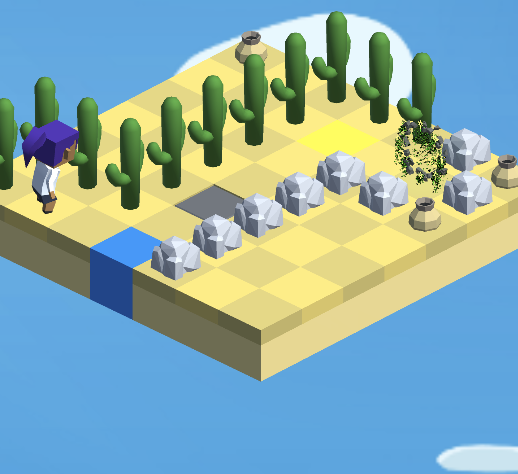
\includegraphics[width=2.5in]{pic-toro/stage/s30.png}
    \end{center}
    \caption[รูปภาพของด่านที่ 30]{รูปภาพของด่านที่ 30}
    \label{s30}
\end{figure}
\pagebreak
\section{Expert evaluation}
การประเมินในด้านระบบของเกม โดยใช้ผู้เชี่ยวชาญในการประเมินคุณภาพอุปกรณ์(เกมเสริมทักษะวิชาวิทยาการคำนวณ) จำนวน 3 ท่าน มีหัวข้อการประเมินประกอบไปด้วย UX/UI ของเกม, ความยากง่ายของเกมเมื่อเทียบกับผู้ใช้ ซึ่งก็คือนักเรียนชั้นประถม
ศึกษาปีที่ 3--6, ผลที่คาดว่าจะสามารถเพิ่มทักษะการคิดอย่างเป็นขั้นเป็นตอนให้กับเด็ก และระบบของเกมโดยรวม ซึ่งประกอบไปด้วย 
การลื่นไหลของ animation, ความเร็วในการตอบสนองของเกม (ไม่มี delay), ไม่พบ error ของระบบ (เด้งหรือค้าง)

\subsection{IOC: Index of item objective congruence}
ผู้พัฒนาได้ใช้โมเดล IOC ซึ่งจะถูกกล่าวในภาคผนวก~\ref{app1} ในการทดสอบวัดคุณภาพของเครื่องมือ(เกมเสริมทักษะวิชาวิทยาการคำนวณ) ซึ่งผู้เชี่ยวชาญจะ
ประเมินแต่ละหัวข้อด้วย 3 ตัวเลือกซึ่งก็คือ ผ่าน, ไม่ทราบ, และไม่ผ่าน ซึ่งการที่ผู้เชี่ยวชาญจะให้ผ่านหรือไม่นั้นเป็นการตีความเองของผู้เชี่ยวชาญ
โดยที่ในแต่ละหัวข้อจะสามารถผ่านได้เมื่อค่าเฉลี่ยในการเลือกให้ผ่านเป็นค่า 66.7\% กล่าวคือในแต่ละหัวข้อต้องถูกประเมินให้ผ่าน 2 ใน 3 ของจำนวนผู้เชี่ยวชาญ โดยมีผลลัพธ์ตามตารางที่~\ref{experteval}
\begin{table}[H]
    \begin{center}
        \begin{tabularx}{\textwidth}{ |>{\raggedright}X*{3}{|l}| }
            \hline
            หัวข้อการสอบถาม & ผู้เชี่ยวชาญคนที่ 1 & ผู้เชี่ยวชาญคนที่ 2 & ผู้เชี่ยวชาญคนที่ 3\\
            \hline\hline
            ความเหมาะสมทางด้าน UX & ผ่าน & ผ่าน & ผ่าน\\
            \hline
            ความเหมาะสมทางด้าน UI & ผ่าน & ไม่ทราบ & ผ่าน\\
            \hline
            นักเรียนชั้นประถมศึกษาชั้นปีที่ 3--6 สามารถเล่นเกมนี้ได้ & ผ่าน (ได้) & ผ่าน (ได้) & ผ่าน (ได้)\\
            \hline
            ตัวเกมสามารถช่วยเพิ่มทักษะการคิดอย่างเป็นขั้นเป็นตอนได้ & ผ่าน (ได้) & ผ่าน (ได้) & ผ่าน (ได้)\\
            \hline
            ตัวระบบโดยรวมของเกมการลื่นไหลของ animation, ความเร็วในการตอบสนอง (ไม่ delay), ไม่พบ error ของระบบ (เด้ง/ค้าง) & ผ่าน & ผ่าน & ไม่ทราบ\\
            \hline
        \end{tabularx}
    \end{center}
    \caption{ตารางผลการประเมินของผู้เชี่ยวชาญ}
    \label{experteval}
\end{table}
จากการวัดคุณภาพของเครื่องมือ (เกมเสริมทักษะวิชาวิทยาการคำนวณ) สรุปได้ว่าทุกหัวข้อนั้นได้ผ่านเกณฑ์ของเครื่องมือวัด IOC ทั้งหมด และเป็นที่น่าพึงพอใจสำหรับผู้เชี่ยวชาญ
% โดยที่สามารถเป็นที่\CI{รองรับ}{??}ได้ว่าตัวเครื่องมือนี้สามารถนำไปใช้ในการพัฒนาทักษะวิชาวิทยาการคำนวณ และการคิดอย่างเป็นขั้นเป็นตอนของเด็กนักเรียนได้อย่างมีประสิทธิภาพ


